\section{Formalization}
\label{sec:formalization}

\subsection{Intermediate Representation}
\label{subsec:ir}

A behavioral synthesis tool performs a number of compiler
and scheduling transformations (including pipelining). Certification of behavioral synthesis transformations thus requires a formalization of
the design representation manipulated by these
transformations. The formalization we use is {\em Clocked
  Control Data Flow Graph} (CCDFG)~\cite{rhcxy:atva-09}. 
Structurally, a CCDFG is a control and data flow graph augmented with a schedule. The control flow is broken into basic blocks. The instructions are grouped into microsteps which can be executed concurrently. A scheduling step represents a group of microsteps which can be executed in a single clock cycle. State of a CCDFG at a particular microstep is a list of all the variables of a CCDFG with their corresponding values. 

The semantics of CCDFG require a formalization of the
underlying language used to represent the individual
instructions in a scheduling step.  The underlying language we use
is the LLVM language~\cite{llvm}. LLVM is a popular compiler
infrastructure for many behavioral synthesis tools
({\em e.g.}, AutoESL~\cite{autoesl}, xPilot~\cite{xpilot}).  We provide semantics to these
instructions through a standard, state-based operational
formalization~\cite{McCarthy}. It includes assignment,
load, store, bounded arithmetic, bit vectors, arrays, and
pointer manipulation instructions. Executing a microstep in
a CCDFG implies changing the current state of CCDFG based on
meaning of the instructions in the microstep and producing a
new state. Assigning meanings to most instructions is
standard; one exception is the so-called ``$\phi$-construct''. A $\phi$-construct is a list of $\phi$-statements. A $\phi$-statement is $v := \phi [\sigma, X] [\tau, Y]$, where $v$ is a variable, $\sigma$
and $\tau$ are expressions, and $X$ and $Y$ are
scheduling steps: if it is reached from $X$ then it is the
same as the assignment statement $v := \sigma$; if
reached from $Y$, it is the same as $v := \tau$; the meaning is undefined otherwise. $\phi$-constructs are necessary due to the structure of the SSA (static single
assignment) form of the LLVM code.

\subsection{Loop Pipelining Transformation}
\label{subsec:loop-pipelining-trans}
A behavioral synthesis tool automatically generates a RTL design from an ESL design through a series of
transformations. Pipelining a loop is a critical
transformation in behavioral synthesis. For our purposes,
{\em pipelinable loop} is a loop with the following additional restrictions~\cite{hrx:dac-12}:
\begin{enumerate}
\item no nested loop;
\item only one $Entry$ and one $Exit$ block; and
\item no branching between the scheduling steps.
\end{enumerate}
These restrictions reflect the kind of loops that can be
actually pipelined during behavioral synthesis. For
instance, synthesis tools typically require inner loops to
have been fully unrolled  in order to pipeline the outer loop.


\begin{figure}[H]%[t!]
\begin{center}
\begin{tabular}{cc}
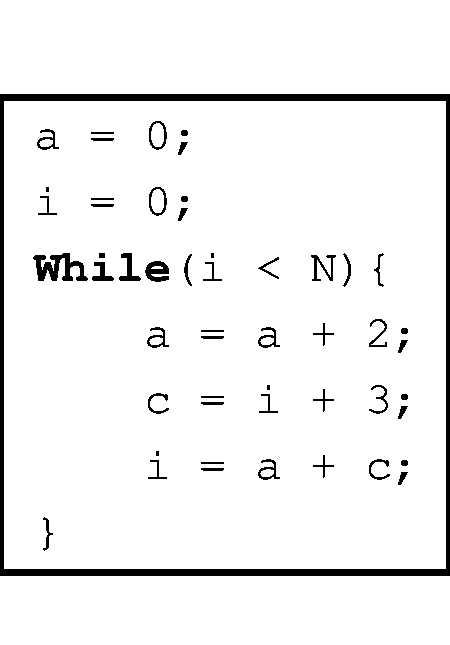
\includegraphics[height=1.5in]{fig-rpe/C-code}
& \hspace{2cm}
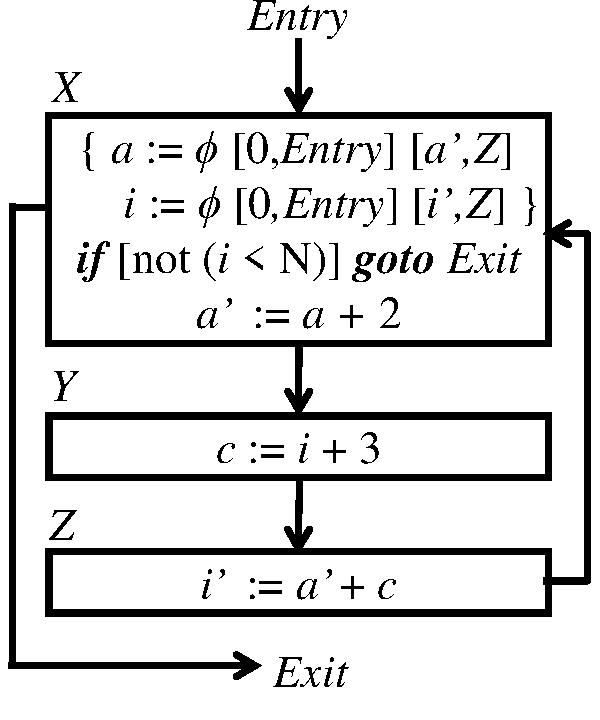
\includegraphics[height=1.5in]{fig-rpe/seq-ccdfg}
\\
(a) & \hspace{2cm} (b) 
\end{tabular}
\end{center}
\caption{(a) Loop in C (b) Loop CCDFG before pipelining.}
\label{fig:high-level-synthesis}
\end{figure}

Figure~\ref{fig:high-level-synthesis}(a) illustrates the C
code for a loop at the beginning of the
synthesis process. The C code does not have a schedule or the
concept of a clock cycle. Figure~\ref{fig:high-level-synthesis}(b)
shows CCDFG of the sequential loop just before loop pipelining. The loop has three scheduling steps: $X$, $Y$ and $Z$.  The scheduling step before the loop is $Entry$ and after the loop is $Exit$. Since,
there are three scheduling steps in the loop, one iteration
can be executed in three clock cycles.

\begin{figure}
\begin{center}
\begin{tabular}{cc}
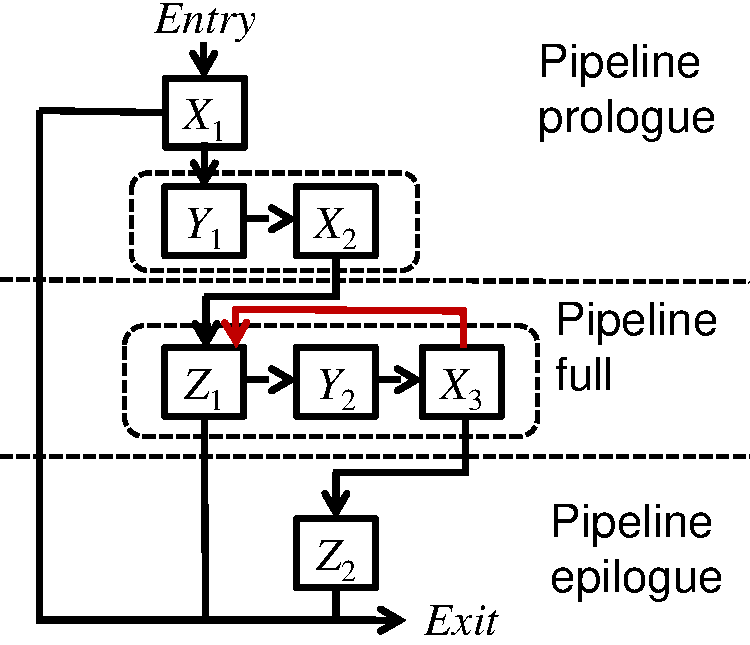
\includegraphics[height=1.5in]{fig-rpe/pipelined_ccdfg}
& \hspace{0.5cm}
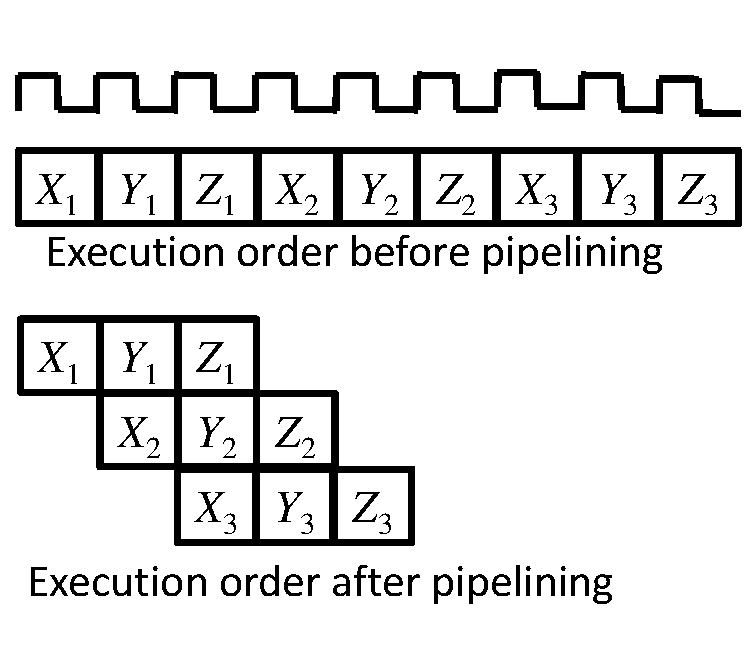
\includegraphics[height=1.5in]{fig-rpe/pp-clock-cycles}
\end{tabular}
\end{center}
\caption{Pipelined CCDFG. The horizontal arrows indicate data forwarding.}
\label{fig:pp-ccdfg}
\end{figure}

Behavioral synthesis tools use complicated heuristics and aggressive scheduling strategies to find an optimized pipeline interval (clock cycles after which a new iteration can be started such that there are no data hazards). Figure~\ref{fig:pp-ccdfg} shows the pipelined CCDFG with a pipeline interval equal to one. The new scheduling steps in the pipelined CCDFG created by combining scheduling steps from different iterations of the sequential CCDFG are called scheduling supersteps. Observe that the three iterations of the pipelined loop take five clock cycles as opposed to nine clock cycles in the sequential loop. Loop pipelining reduces the number of clock cycles required to execute the loop, hence this transformation is used by synthesis tools to increase throughput and reduce latency.  

\subsection{Correctness of Pipelined CCDFG}
\label{subsec:correctness-defn}

Loop Pipelining is a critical and complex transformation. So, it is important to certify that the pipelined CCDFG is indeed correct. Correctness of loop pipelining can be informally stated as below.

\begin{quote}
Let $L$ be a loop in CCDFG $C$, and let $L_{\alpha}$ be the
pipelined loop CCDFG. Let $V$ be the set of
variables mentioned in $L$, and $U$ be the set of all
variables in $C$.  Suppose we execute $L$ and $L_{\alpha}$
from CCDFG states $s$ and $s'$ respectively, such that for
each variable $v\in V$, the value of $v$ in $s$ is the same
as that in $s'$, and suppose that the state on termination
are $f$ and $f'$ respectively.  Then (1)~for any $v\in V$,
the value of $v$ in $f$ is the same as that in $f'$, and
(2)~for any $v\in(U\backslash V)$, the value of $v$ in $f'$
is the same as that in $s'$.
\end{quote}
\noindent
{\em Remark:} Condition (2) is the {\em frame rule} which
ensures that variables in $C$ that are not part of the loop
are not affected by $L_{\alpha}$.

